
\section{Experimental Results}

The experimental evaluation carried out with UPsCAle was divided into two parts. First we evaluate the semantic topics extracted by the method proposed in Section~\ref{sec:merge} using two labelled datasets. Next we show a case study on a Twitter dataset that considers the followers of Obama and their messages posted during the presidential election campaign in 2012, assessing the full extension of UPsCALe. 
Table~\ref{tbl:datasets} shows the main characteristics of the three datasets considered. 
%AgNews is a collection of articles from the AG news corpus published daily. The news articles have been gathered from more than 2,000 news sources by an academic search engine: \textit{ComeToMyHead} \cite{newEngine}. 
In order to simulated a scenario with restricted contextual information, as in social media posts, for AgNews we consider only the titles from each news in this collection to associate the documents with the 11 classes. 
The second labelled dataset is the Observatory, composed by a set of 6,000 tweets collected using keywords and manually classified as belonging to one out of six topics: religion, dengue fever, soccer, election, traffic, or cars.


\subsection{Semantic Topic Identification}

This section describes the topic identification evaluation followed by the results for topic identification in the two labelled datasets.

\subsubsection{Evaluation Methodology}

Evaluating the topics identified by \method can be as difficult as obtaining them. For this reason, this section defines a set of metrics that, given a known set of topics, evaluates the performance of the semantic topic identification phase. Consider we are 
interested in finding semantic topics that present high representativeness, high cohesion and low 
fragmentation (uniqueness).
The representativeness of the topics is currently given as a parameter to the system, and used by PCA to define the number 
of latent factors we are looking for. In the experiments, different results of representativeness 
were tested and a subset of them is presented in this section. For cohesion and uniqueness, we defined the following metrics.

Cohesion, or the intra-clustering similarity, is measured using the purity of the semantic topics found \cite{witten:2005}. In order to calculate purity, each semantic topic is paired with the most frequent class in the documents of the topic, and then the accuracy is measured by counting the number of correctly assigned documents over the total number of documents, as showed in Eq.~\ref{eq:purity}. 
$T$ represents the sets of semantic topics (clusters) found, $C$ is the set of real, known topics (or classes), and D the total number of tweets. 

\vspace{-0.3cm}
\begin{equation}
\label{eq:purity}
purity(T,C) = \frac{1}{D}\sum_{i=0}^k{max_j|t_i \cap c_j|}.
\end{equation}
\vspace{-0.3cm}

Fragmentation, in turn, measures the inter-clustering 
similarity using the {\sc MRVI} (\textit{Mean Relative Vocabulary Intersection}) \cite{kao2004mining}
among pairs of topics $T_i$ and $T_j$. The intuition behind this metric is that if $T_j$ is a subset of 
$T_i$, then the vocabulary intersection between samples of $T_j$ and $T_i$ with the complete set $T_i$ are similar. A global fragmentation analysis is done by plotting the distribution of MRVI among all pairs of topics $T_i, T_j \in T$. The higher the $RVI$ the higher the probability 
of $T_j$ being a fragment of $T_i$.

\begin{table}[t]
\begin{scriptsize}
\caption{Datasets used by \method to extract semantic topics} \label{tbl:datasets}
    \begin{center}
	\begin{tabular}{|c|c|c|c|c|c|}
	    \hline 
	    Dataset        & Users &\#Posts & \#Topics & \#Terms \\ \hline
	    \hline
%	    LouisVuitton   &  641,302 & - & &  \\ \hline
	    AgNews         &  -&878,705 & 5       & 99,394 \\ \hline
	    Observatory &  -&5,431  & 6       &1,956 \\ \hline
	    USAElections   &  53,571&708,121& - &  61,526 \\ \hline
	\end{tabular}
    \end{center}
\end{scriptsize}
\end{table}

%Suppose we want to calculate the $MRVI$ of $T_j$ with respect to $T_i$. Let $D^{T_i}$ and $D^{T_j}$ be subsets of documents from $D$ that had topics $T_i$ and $T_j$ assigned to them, respectively. First, we sample two subsets $D^{T_i}_S$ and $D^{T_j}_S$ from $D^{T_i}$ and $D^{T_j}$, respectively, by randomly selecting $L$ distinct documents.  We define $L$ as the third part of the smallest of the subsets $D^{T_i}$ and $D^{T_j}$. Then, we determine the vocabulary intersection between $D^{T_i}$ and $D^{T_i}_{S}$ and again between $D^{T_i}$ and $D^{T_j}_{S}$, defining intersection measures $I(T_i,T_i)$ and $I(T_i,T_j)$ using the Jaccard metric. Next, the relative vocabulary intersection $RVI$ is defined as the rate between  $I(T_i,T_i)$ and $I(T_i,T_j)$. Therefore, the higher the $RVI$ the higher the probability of $T_j$ being a fragment of $T_i$. We repeat this process $n$ times generating distinct samples $D^{T_i}_S$ and $D^{T_j}_S$, and define the MRVI as the mean of the RVI over $n$ executions. A global fragmentation analysis is done by plotting the distribution of MRVI among all pairs of topics $T_i, T_j \in T$.



% \begin{figure*}[!th]
% \centering
% \subfigure[AgNews]{{file=figures/topicDistributionAgnews.eps,width=1.53in,height=1.13in}} \quad
% \subfigure[Observatory]{{file=figures/topicDistributionObservatory.eps, width=1.53in,height=1.13in}}
% \subfigure[AgNews]{{file=figures/numTopicsPerDocAgNews.eps, height=1.53in,width=1.13in,angle=-90}}
% \subfigure[Observatory]{{file=figures/numTopicsPerDocObservatory.eps, height=1.53in,width=1.13in,angle=-90}}
% \caption{Topics most frequently assigned to documents (a) and (b), and the average number of topics assigned per document (c) and (d) for both agNews and Observatory}
% \label{fig:histograms}
% \end{figure*}


Apart from the two aforementioned metrics, we also calculate the precision and recall of the topics. The way precision and recall are calculated depend on how the documents are mapped to topics found and how topics are mapped to the known classes. Recall that a post can be associated with zero, one or more topics. Similarly, a topic can be mapped to one or more classes.
Hence, when precision and recall are calculated, they consider only the documents that belong to at least one topic. For this reason, we refer to the precision and recall metrics as an ``estimated" precision and recall, or e-precision and e-recall. 

The evaluation measures showed here were calculated under four scenarios. The first, named 1-1\_1-1, maps one document to one topic, and one topic to one class. This is the most restrictive metric, which associates the document with the most probable topic and the topic with the most frequent class among the documents in that topic. The second, 1-1\_N-1, maps one document to one topic but $n$ topics to one class. In this case, classes may refer to more than one topic. The third measure allows one document to be mapped to more than one topic, and again more than one topic may be associated with a single class (1-N\_N-1). Finally, the less restrictive metric is 1-N\_N-N, which maps one document to $n$ topics, and these $n$ topics with $n$ classes, characterizing a multi-label class problem.
For the first three cases, e-precision and e-recall are calculated using the tradition precision formula \cite{witten:2005}. For the fourth case, a multi-label version of these metrics is used \cite{tsoumakas2007multi}. 

In cases where the number of topics found is greater than the number of actual classes, depending on which type of topic-class mapping is being used, only the topics with the highest number of documents are mapped to the real classes, and this is reflected in the recall of the methods. 
\begin{figure}[!t]
%	\subfigure{
%		\begin{minipage}[c]{.05\textwidth}
%		\end{minipage}
%		\begin{minipage}[c]{.95\textwidth}
%			\hspace{2.3cm}
%			\begin{scriptsize} \textbf{AgNews} \end{scriptsize} 
%			\hspace{2.6cm}
%			\begin{scriptsize} \textbf{Observatory} \end{scriptsize}
%		\end{minipage}
%	}\\
%	\subfigure{
%		\begin{minipage}[c]{.05\textwidth}
%			\vspace{-0.7cm}
%			\hspace{-0.6cm}
%			\centering
%				\begin{sideways}
%					\begin{scriptsize} \textbf{Freq. Assigned Topics} \end{scriptsize}
%				\end{sideways}
%		\end{minipage}
%		\begin{minipage}[c]{.45\textwidth}
%		\vspace{-0.4cm}
%		\hspace{-0.5cm}
%		\centering
%		\subfigure{{file=figures/topicDistributionAgnews.eps,width=1.53in,height=1.13in}}
%		\subfigure{{file=figures/topicDistributionObservatory.eps, width=1.53in,height=1.13in}}
%		\end{minipage}
%	}
	\subfigure{
		\begin{minipage}[c]{.05\textwidth}
			\vspace{-0.6cm}
			\hspace{-0.6cm}
			\centering
			\begin{sideways}
				\begin{scriptsize} \textbf{Avg number of topics} \end{scriptsize}
			\end{sideways}
		\end{minipage}
		\begin{minipage}[c]{.43\textwidth}
			\vspace{-0.4cm}
			\hspace{-0.5cm}
			\centering
			\subfigure{{file=figures/numTopicsPerDocObservatory, height=1.53in,width=1.13in,angle=-90}}
			\subfigure{{file=figures/numTopicsPerDocAgNews, height=1.53in,width=1.13in,angle=-90}}

		\end{minipage}
	}
%%	\vspace{-0.3cm}
	\caption{Topics most frequently assigned to documents %(a) and (b), and the average number of topics assigned per document (c) and (d) 
	for Observatory and agNews}
	\label{fig:histograms}
\end{figure}

Considering these metrics, \method is compared with three other semantic topic identification techniques. The first, NMF, corresponds to the first part of \method and does not perform any merging of topics after finding the latent factors. The second applies a hierarchical average-linkage clustering algorithm to the topics extracted using Singular Value Decomposition (SVD), as done in \cite{kuhn2007semantic}. A version of Matlab's hierarchical clustering algorithm was used. Finally, the third method applies the expectation-maximization algorithm %(Weka version \cite{witten:2005}) 
to the topics created by NMF to merge topics. In this case, instead of using the $PCA$ to find the number of latent factors needed for a given representation, we use a predefined number of latent factors defined by the formula given in \cite{kuhn2007semantic}. A second version of this baseline, replacing NMF by SVD was also tested, and the results were statistically worst than those reported here.
For all baselines, the mapping between topics and classes follows the same principles as for UPsCALe. NMF runs for 100 iterations in all
cases.


\subsubsection{Experimental Results}

For the two labelled datasets, AgNews and Observatory, we report a subset of tests with different levels of topics representativeness (35\%, 45\% and 55\%) and $\alpha$ (0.3 and 0.5). % and 0.7.) 
As the topic-document mapping plays an important role during evaluation, Figure~\ref{fig:histograms} shows %the cumulative distribution function (CDF) for the most frequently assigned topics. %, and 
the number of documents to which 1, 2 and 3 topics were assigned. The analysis shows that no more than 3 topics were assigned to any document in both datasets. As data representativeness increases and reaches 55\% the number of documents assigned to more than two topics increases, but all baselines considered are assigned only one topic per document. Note that the values for SVD-HC and NMF+EM are not shown for agNews because they present a prohibitive computational time. \looseness=-1


Table~\ref{tbl:topics} shows the average results obtained over 10 runs of the methods. Results are compared using a two-tailed t-test with significance level 0.95. The second column shows the method considered: UPsCAle, SVD+HC, NMF+EM and NMF. For the latter, the number of latent factors to be found ($k$) is set as the number of known topics. In the case of UPsCAle, it is followed by the data representativity required (given as a parameter to PCA, which returns $k$). When the value of representativeness is missing, $k$ is set to $(m \times n)^2$ \cite{kuhn2007semantic}. The next two columns, under the name \# Topics, show the number of topics returned by PCA ($k$) followed by the final number of topics, obtained after running the merging phase of UPsCAle ($k'$). Note that, for AgNews, although the initial number of given topics was 12, this value decreased to 5 after the document-topic mapping, as documents belonging to 7 different small classes did not belong to any topics. The next column, Docs with Topics, shows the fraction of documents which were assigned to at least one topic. We emphasize that the metrics of e-precision and e-recall for the four situation previously described provided in the next columns were calculated over these documents.

\begin{figure}[!tb]
 \centering
 \subfigure[Observatory]{{file=figures/topicsFragmentationObservatory.eps,height=1.4in,width=1.5in}}
% \subfigure[Observatory]{{file=figures/fragmentation-Observatory-KT.eps, width=1.8in,height=1.45in}}
% \subfigure[Observatory]{{file=figures/fragmentation-Observatory-CL.eps, width=1.8in,height=1.45in}}
% \subfigure[AgNews]{{file=figures/fragmentation-agnews-upscale.eps,width=1.8in,height=1.45in}} %0.35
 \subfigure[AgNews]{{file=figures/topicsFragmentationAgNews.eps,height=1.4in,width=1.5in}}
 \caption{Distribution of $MRVI$ among all pairs of topics}
 \label{fig:mrvi}
 \end{figure}

In general, we observe that the higher the representativeness, the higher the number of covered examples, as more topics cover more documents. Similarly, the higher the value of cohesion, the higher the number of final topics $k'$, as the topics become more fragmented to be more cohesive. The differences between $k$ and $k'$ show that the merging process proposed significantly reduces the number of topics found.
In average, the proposed method performed 19 iterations for Observatory and 29 to AgNews.


Now looking at the Observatory dataset. 
The number of documents assigned to at least one topic varied from 88 to 99\% according to different representativeness.
When the number of topics was previously set, this number decreased to 40\%. 
In order to analyse precision and recall, we select one of the results and compare it against the others using the t-test. The results compared are highlighted in gray, and the symbol \textcolor[rgb]{00,0.45,0.10}{$\blacktriangle$} in a cell indicates its result is better than the highlighted, \textcolor[rgb] {0.7,00,00}{$\blacktriangledown$} indicates it is worse and \textcolor[rgb]{0.7,0.7,0.0}{$\bullet$} that there is no statistical evidence to state any difference.


%\newcommand{\green}{\cellcolor{green}}
%\newcommand{\red}{\cellcolor{red}}
%\newcommand{\norm}{\cellcolor{blue}}

\newcommand{\green}{\textcolor[rgb]{00,0.45,0.10}{$\blacktriangle$}}
\newcommand{\red}{\textcolor[rgb] {0.7,00,00}{$\blacktriangledown$}}
\newcommand{\norm}{\textcolor[rgb]{0.7,0.7,0.0}{$\bullet$}}




\begin{sidewaystable}
%\begin{table*}
%\begin{scriptsize}
\caption{ Results obtained for Observatory and AgNews. Documents with topics represent the number of documents assigned to at least one topic. The metrics of precision and recall are calculated under these documents. The four cenarious presented considering different mapping of Doc\_Topic\_Topic\_Class. \\}
\label{tbl:topics}



\begin{tabular}{|c||c|c|c|c||c|c|c|c|c|c|c|c|c|}
\hline
Cohesion&\multirow{2}{*}{Method}&\multicolumn{2}{c|}{\#Topics}&Docs &\multirow{2}{*}{Purity}&\multicolumn{2}{c|}{1-1\_1-1} &\multicolumn{2}{c|}{1-1\_N-1} &\multicolumn{2}{c|}{1-N\_N-1} &\multicolumn{2}{c|}{1-N\_N-N}\\ \cline{3-4}\cline{7-14}
         	($\alpha$) &          &     k    &      k'       & with Topics    &  & e-prec.   & e-recall          & e-prec.   & e-recall          & e-prec.   & e-recall          & e-prec.   & e-recall          
\\ \hline \hline

 \multicolumn{14}{|c|}{\textbf{Observatory}} 
\\ \hline \hline

\multirow{4}{*}{0.30} 
  & UPsCAle-0.35 & 115& 15.6 & \red 0.883 & \red 0.641 & \red 0.574 & \green 0.380 & \norm  0.477 & \green 0.435 & \norm  0.437 & \green 0.466 & \norm 0.789 & \green 0.884
\\ 
 & UPsCAle-0.45 & 171& 23.3 & \red 0.968 & \red 0.678 & \red 0.579 & \green 0.280 & \norm 0.461 & \green 0.358 & \norm 0.422 & \green 0.395 & \red 0.757 & \red 0.863
\\ \index{•}
 & UPsCAle-0.55 & 242& 31.3 & \norm 0.995 & \red 0.685 & \red 0.554 & \green 0.217 & \norm 0.451 & \green 0.304 & \norm 0.406 & \green 0.342 & \red 0.753 & \norm 0.873
\\
& UPsCAle & 25 & 5.9 & \red 0.391 & \green 0.825 & \red 0.520 & \green 0.429 & \norm  0.494 & \green 0.450 & \green 0.476 & \green 0.455 & \green 0.852 & \norm 0.868
\\ \hline{}

\multirow{4}{*}{0.50} 
 & UPsCAle-0.35 & 115& 25.1   & \red 0.885 & \red 0.696 & \red 0.582 & \green 0.283  & \green 0.473 & \green 0.364  & \norm 0.434 & \green 0.390  & \norm 0.769 & \red 0.855  
\\
 & UPsCAle-0.45 & 171 & 32.9  & \red 0.963 & \red 0.698 & \norm  0.631 & \green 0.244  & \norm 0.461 & \green 0.326  & \norm 0.413 & \green 0.363  & \red 0.761 & \red 0.864  
\\ 
 & \multicolumn{1}{| >{\cellcolor[gray]{0.85}}c|}{UPsCAle-0.55} & \multicolumn{1}{| >{\cellcolor[gray]{0.85}}c|}{242}& 
 \multicolumn{1}{| >{\cellcolor[gray]{0.85}}c|}{43.9}    & \multicolumn{1}{| >{\cellcolor[gray]{0.85}}c|}{0.995} & 
 \multicolumn{1}{| >{\cellcolor[gray]{0.85}}c|}{0.745} &  \multicolumn{1}{| >{\cellcolor[gray]{0.85}}c|}{0.657} & 
 \multicolumn{1}{| >{\cellcolor[gray]{0.85}}c|}{0.175}  & \multicolumn{1}{| >{\cellcolor[gray]{0.85}}c|}{0.438} & 
 \multicolumn{1}{| >{\cellcolor[gray]{0.85}}c|}{0.247}  & \multicolumn{1}{| >{\cellcolor[gray]{0.85}}c|}{0.404} & 
 \multicolumn{1}{| >{\cellcolor[gray]{0.85}}c|}{0.271}  & \multicolumn{1}{| >{\cellcolor[gray]{0.85}}c|}{0.773} & 
 \multicolumn{1}{| >{\cellcolor[gray]{0.85}}c|}{0.873}
 \\
 & UPsCAle & 25 & 9.7    & \red 0.395 & \norm 0.747 & \norm 0.631 & \green 0.442  & \green 0.566 & \green 0.508  & \green 0.552 & \green 0.516 & \green 0.859 & \norm 0.883

\\ \hline	


%\multirow{4}{*}{0.70} 
% & UPsCAle-0.35 & 115& 29.9 & \red 0.889 & \red 0.682 & \norm 0.655 & \green 0.288 & \green 0.513 & \green 0.398 & \green 0.466 & \green 0.430 & \norm 0.768 & \red 0.855
%\\ 
% & UPsCAle-0.45 & 171& 38.1 & \red 0.967 & \red 0.699 & \norm 0.622 & \green 0.218 & \norm 0.448 & \green 0.315 & \norm 0.412 & \green 0.348 & \norm 0.775 & \norm 0.873
%\\ 
% & UPsCAle-0.55 & 242& 43.7 & \norm 0.995 & \norm 0.745 & \norm 0.623 & \norm 0.179 & \norm 0.458 & \green 0.261 & \norm 0.399 & \green 0.284 & \green 0.810 & \green 0.907 
%\\
%& UPsCAle  & 25 & 17.2 & \red 0.399 & \red 0.602 & \norm  0.732 & \red 0.405 & \green 0.653 & \green 0.645 & \green 0.642 & \green 0.657 & \green 0.830 &  0.865
%\\ \hline 


\multirow{4}{*}{-} 
 & SVD+HC & - &2,333 & \green 0.999 & \red 0.354 & \green 0.898 & \red 0.024 & \green 0.776 & \green 0.775 & \green 0.776 & \green 0.775 & \green 0.956 & \green 0.956
\\ 
 & NMF+EM & 25 & 12.7 & \red 0.925 & \red 0.540 & \red 0.435 & \green 0.289 & \norm 0.390 & \green 0.415 & \norm 0.390 & \green 0.415 & \green 0.812 & \red 0.812
\\ 
 & NMF & 6 & 6.0 & \red 0.111 & \green 0.780 & \norm 0.670 & \green 0.629 & \green 0.671 & \green 0.699 & \green 0.669 & \green 0.700 & \green 0.921 & \green 0.923  
\\ \hline	


\hline

\multicolumn{14}{|c|}{\textbf{AgNews}} 
\\ \hline \hline
 
 \multirow{3}{*}{0.30} 
  & UPsCAle-0.35 & 59&  13.9 & \red 0.011 & \red 0.559 & \red 0.181 & \green 0.191 & \red 0.200 & \green 0.204 & \norm 0.200 & \green 0.204 & \norm 0.763 & \green 0.836
\\ 
 & UPsCAle-0.45 & 103& 19.4 & \red 0.085 & \red 0.694 & \red 0.242 & \green 0.166 & \norm 0.206 & \green 0.181 & \norm 0.207 & \green 0.186 & \green 0.781 & \green 0.806
\\ 
 & UPsCAle-0.55 & 163& 31.9 & \norm 0.359 & \norm 0.803 & \norm 0.246 & \norm 0.125 &  \norm 0.212 & \norm 0.137 & \norm 0.197 & \norm 0.140 & \norm 0.762 & \norm 0.797
\\
& UPsCAle        & 154 & 29.5 & \norm 0.283 & \norm 0.796 & \red 0.242 & \green 0.143 & \norm 0.212 & \norm 0.154 & \norm 0.189 & \norm 0.154 & \green 0.765 & \green 0.796 
\\ \hline{}


\multirow{3}{*}{0.50} 
 & UPsCAle-0.35 & 59& 16.5   & \red 0.011 & \red 0.557 &  \red 0.229 & \green 0.219  & \norm 0.227 & \green 0.238  & \norm 0.231 & \green 0.239  & \green 0.784 & \green 0.855
\\
 & UPsCAle-0.45 & 103 &  24.1  & \red 0.090 & \red 0.693 & \norm  0.309 & \green 0.183  & \norm 0.256 & \green 0.202  & \norm 0.248 & \green 0.207  & \green 0.776 & \green 0.802
\\ 
 

 & \multicolumn{1}{| >{\cellcolor[gray]{0.85}}c|}{UPsCAle-0.55} & \multicolumn{1}{| >{\cellcolor[gray]{0.85}}c|}{163}& 
 \multicolumn{1}{| >{\cellcolor[gray]{0.85}}c|}{34.4}    & \multicolumn{1}{| >{\cellcolor[gray]{0.85}}c|}{0.360} & 
 \multicolumn{1}{| >{\cellcolor[gray]{0.85}}c|}{0.810} &  \multicolumn{1}{| >{\cellcolor[gray]{0.85}}c|}{0.292} & 
 \multicolumn{1}{| >{\cellcolor[gray]{0.85}}c|}{0.117}  & \multicolumn{1}{| >{\cellcolor[gray]{0.85}}c|}{0.252} & 
 \multicolumn{1}{| >{\cellcolor[gray]{0.85}}c|}{0.132}  & \multicolumn{1}{| >{\cellcolor[gray]{0.85}}c|}{0.235} & 
 \multicolumn{1}{| >{\cellcolor[gray]{0.85}}c|}{0.137}  & \multicolumn{1}{| >{\cellcolor[gray]{0.85}}c|}{0.751} & 
 \multicolumn{1}{| >{\cellcolor[gray]{0.85}}c|}{0.783}
 \\
 
 
 
 
 & UPsCAle & 154 &   31.9   & \norm 0.283 & \red 0.787 & \norm 0.304 & \green 0.139  & \norm 0.245 & \green 0.157 & \norm 0.228 & \green 0.165  & \green 0.770 & \green 0.799 
\\ \hline

%\multirow{3}{*}{0.70} 
% & UPsCAle-0.35 & 59& 38.3 & \red 0.011 & \red 0.335 & \norm 0.413 & \green 0.328 & \green 0.388 & \green 0.394 & \green 0.382 & \green 0.387 & \green 0.790 & \green 0.882
%\\ 
% & UPsCAle-0.45 & 103& 56.7 & \red 0.085 & \red 0.468 & \green 0.471 & \green 0.235 & \green 0.419 & \green 0.354 & \green 0.419 & \green 0.358 & \green 0.777 & \green 0.819
%\\ 
% & UPsCAle-0.55 & 163& 42.1 & \norm 0.341 & \red 0.741 & \green 0.382 & \green 0.180 & \green 0.321 & \green 0.206 & \green 0.299 & \green 0.215 & \green 0.775 & \green 0.815
%\\
%& UPsCAle       & 154 & 39.1 & \norm 0.283 & \red 0.743 & \green 0.387 & \green 0.194 & \green 0.316 & \green 0.217 & \green 0.305 & \green 0.225 & \green 0.787 & \green  0.822
%\\ \hline
- & NMF & - & 11 & - & - & - & - & - & - & - & - & - & - 
\\ \hline

\end{tabular}



%\end{scriptsize}
%\end{table*}

\end{sidewaystable}












Analysing the precision and recall, \method with $\alpha=0.5$ and 0.55 representativeness was chosen as a reference, as it will cover more documents and set an equal trade-off for cohesion and uniqueness. Comparing these results with the other using $\alpha=0.3$, for all e-precisions except the most restrictive, the results found are better than the reference. Looking at the baselines, the results of SVD+HC seem far better than those obtained by UPsCAle. However, note that SVD+HC found 2,333 clusters. In the evaluation process, as only six clusters were mapped to the real classes in the 1-1\_1-1 evaluation, the recall is around 2\%, explaining the high precision. NMF also presented a much higher e-precision and e-recall than UPsCAle, but the column ``Docs with Topics" shows that only 11\% of documents were assigned to at least one topic in this case. NMF+EM is the strongest competitor, but given its final number of topics, the fairest comparison is to compare it with UPsaAle-0.35 with $\alpha=0.3$. The latter covers 4\% less documents, but presents higher purity and both e-precision and recall for all mapping, except for the less restrictive precision. Hence, tuning $\alpha$ and the representativeness, we can obtain better results than the current methods more efficiently, as discussed below.  
The much lower purity of NMF+EM might be due to the final number of topics. %However, it corroborates the main criticism against using the number of latent factors defined by \cite{kuhn2007semantic}, which usually requires a small number of latent factors which will usually returned mixed semantic topics.


With respect to agNews, we observe a completely different situation. The cost of the baselines was prohibitive, and when 11 was given to NMF as the number of latent factors to be found (i.e. the number of known-topics), only 57 documents (out of 878,705) were assigned to topics. The values of assignment for \method are also low, reaching 36\% with the highest value of representativeness and 34 topics in average.

The last metric calculated over the labelled datasets, fragmentation, is showed in Figure \ref{fig:histograms}. The histograms for the two datasets are completely different (recall that the lower the MRVI, the better). For Observatory, the graph shows that \method 0.55 is superior, i.e., the topics found overlap less. For agNews, \method using the predefined number of topics is superior, but this is due to the size of the topics (clusters) generated. As they are smaller, they tend to overlap less, and hence MRVI is better. 

\begin{figure*}[!tb]
 \centering
\subfigure[]{
\includegraphics[width=1.6in,height=1.35in]{figures/cloudTags/top1-elections.png}}
\subfigure[]{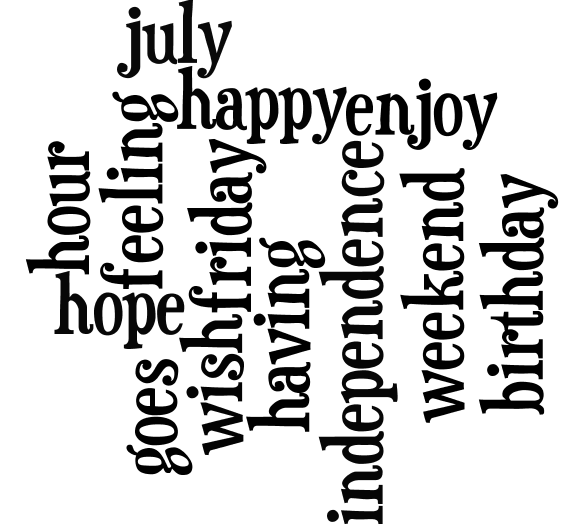
\includegraphics[width=1.6in,height=1.35in]{figures/cloudTags/top2-elections.png}} 
 \subfigure[]{
\includegraphics[width=1.6in,height=1.35in]{figures/cloudTags/top3-elections.png}}
 \subfigure[]{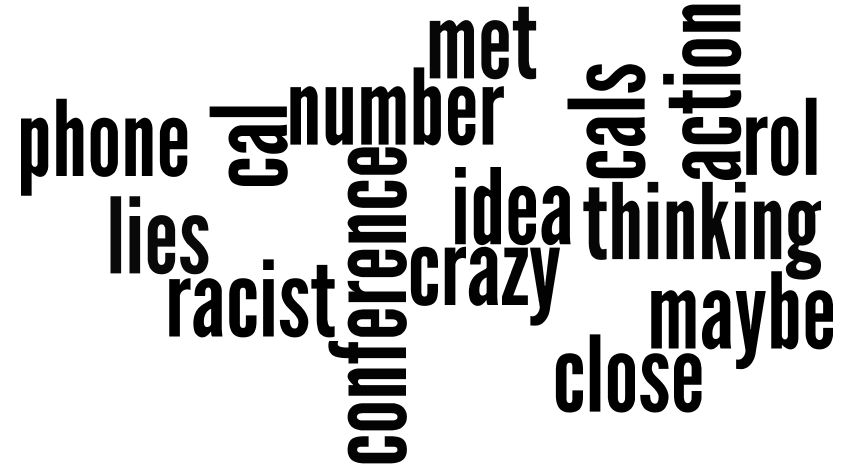
\includegraphics[width=1.6in,height=1.35in]{figures/cloudTags/top6-elections.png}} 
 \caption{Main topics discussed by Obama's followers: Independence Day, Democrats Convention in Sep. 2012 and gay marriage, Congress, and Call for an Ant-Racist Action.}
 \label{fig:election}
  \end{figure*}

\begin{table}[t]
\center
\begin{scriptsize}
\caption{Results obtained by UPsCAle considering Obama's followers in Twitter}\label{tbl:unlabeled}
\begin{tabular}{|l|l|l|l|l|}
\hline
 \multicolumn{5}{|c|}{Obama's Followers}  \\  \hline 
 \multirow{5}{*}{$\alpha$= 0.5} &\multirow{2}{*}{Repres.} & \multicolumn{2}{c|}{\#Topics} & \multirow{2}{*}{Purity}  \\ \cline{3-4}
 & & k & k' & \\ \cline{2-5}
 &0.35 & 94& 40.5 & 0.608 \\ %\cline{2-5}
 &0.45 & 141 & 43.75 & 0.613 \\ %\cline{2-5}
 &0.55 & 204 & 57.67 & 0.629 \\ \hline
%\multirow{3}{*}{FIAT} & \multirow{3}{*}{Framework} & 0,35 & 26 & 0.161 \\ \cline{3-5}
%&  & 0,45 & 47 & 0.144 \\ \cline{3-5}
%&  & 0,55 & 30 & 0.127 \\ \cline{3-5}
%\multirow{3}{*}{LouisVuitton} & \multirow{3}{*}{Framework} & 0,35 & 30 & 0.336 \\ %\cline{3-5}
%&  & 0,45 & 42 & 0.295 \\ \cline{3-5}
%&  & 0,55 & 61 & 0.153 \\ \hline
\end{tabular}
\end{scriptsize}
\end{table}

% \begin{table}
% \begin{tabular}{|l|l|l|l|l|}
% \hline
% Database & Repr & PCA & Clusters & Purity  \\ \hline
% \multirow{3}{*}{Election} & 0,35 & 94&34 & 0.617  --  0.535 \\ \cline{3-5}
% &  0,45 & 141 & 47 & 0.621  --  0.532 \\ \cline{3-5}
% &  0,55 & 204 & 52 & 0.652  --  0.552 \\ \hline
% %\multirow{3}{*}{FIAT} & \multirow{3}{*}{Framework} & 0,35 & 26 & 0.691  --  0.595 \\ \cline{3-5}
% %&  & 0,45 & 47 & 0.659  --  0.576 \\ \cline{3-5}
% %&  & 0,55 & 30 & 0.763  --  0.677 \\ \cline{3-5}
% %\multirow{3}{*}{LouisVuitton} & \multirow{3}{*}{Framework} & 0,35 & 30 & 0.635  --  0.475 \\ %\cline{3-5}
% %&  & 0,45 & 42 & 0.614  --  0.474 \\ \cline{3-5}
% %&  & 0,55 & 61 & 0.660  --  0.572 \\ \hline
% \end{tabular}
% \end{table}
% 


%\begin{table*}
\caption{Textual Description for the top-15 semantic topics identified in datasets agNews and Observatory.}\label{tbl:topicDescriptions}
\centering
	\begin{tiny}
	\begin{tabular}{|p{5.0cm}|p{5.0cm}|}\hline
		\textbf{AgNews}  & \textbf{Observatory} \\ \hline \hline
		
		che, non, con, una, roma, nel, calcio, man, dei, win, season, night, film, country, states  &  love, doctor, improvements, glory, going, strong, hope, world, hospital, night, know, brother, father, body, fever \\ \hline
		fedflare, style, latest, ful, story, both, details, read, display, none, release, version, releases, bok  &  slow, city, forward, thing, cause, brazil, center, hadad, street, look, debate, city, marcelo, height, support \\ \hline
		space, international, nasa, launch, shutle, station, atlantis, mission, astronauts, discovery, crew, agency, cape, canaveral, weather  &  live, earn, gremio, flu, corinthians, time, final, palmeiras, atletico, lose, guarani, goal, bahia, galo, fluminesne \\ \hline
		today, prnewswire, joke, leading, expected, usa, early, leaders, ago, firstcal, solutions, corporation, nbc, event, blockquote  &  with, and, con, new, audi, nissan, dodge, toyota, car, celta, auto, leader, corsa, strada, can \\ \hline
		set, record, fire, sets, start, date, deadline, final, take, loks, expected, anounce, begin, aside  &  back, show, psdb, twiter, follow, internet, win, pair, tickets, asks, civic, close, wake, guys \\ \hline
		plans, cut, sel, build, anounce, europe, largest, move, buy, part, corp, plant, cuts, expand, production  &  car, leaves, uno, music, advertising, caught, listen, telo, michel, like, commercial, santana, luan, success, thanks \\ \hline
		way, page, articlebody, our, used, fol, change, social, want, paving, fast, very, find, going, around  &  vasco, week, video, national, gama, \#euteamovasco, passed, earth, volleyball, shopping, visiting, ministry, praise, sea \\ \hline
		big, east, smal, brother, ten, scren, midle, dig, bowl, made, play, conference, money, much, another  &  makes, mean, kind, bottling, things, like, believer, stopped, santistas, passes, christian, part, chico, eating, \#santos \\ \hline
		through, thousands, weather, snow, riped, spam, strets, rain, swept, tore, another, water, hundreds, across, extension  &  friend, levy, Fidelix, man, mustache, aerotrem, hemorragic, be, party, birthday, minister, nobody, niece, sad, soninha \\ \hline
		anounced, conference, anounces, agrement, leading, prnewswire, global, awards, june, anual, feb, nasdaq, corporation, prize, march  &  saw, bad, beautiful, care, class, pretty, easy, sweetheart, arrives, here, leave, worse, step, wtf, dps \\ \hline
		life, real, prison, long, virtual, family, live, batery, sentenced, half, mars, scientists, insurance, water, bok  &  speech, team, ole, heart, name, fan, imagine, desire, crazy \\ \hline
		stil, despite, long, even, while, missing, though, death, another, remains, much, yet, god, although, ago  &  know, wanted, result, exam, morning, exams, ese \\ \hline
		now, long, ago, available, then, again, once, until, months, going, realy, change, wgc, same, wel  &  sunday, saturday, friday, schedule, guys, next, be, porto-alegre, candidates, grace, coming, friends, flu, decision \\ \hline
		plan, public, sharon, part, safety, proposal, spectrum  &  globe, making, novel, want, record, radio, network, play, teams, minister \\ \hline
		media, reported, chinese, reports, player, beijing, television, times, newspaper, digital, content, comission  &  stay, rain, neymar, give, accept, ring, trapped, missing, elections, place up, start, eat, celso \\ \hline
% 		internet, users, acess, ogi, aol, broadband, net, computer, explorer, ban, chinese, fre, browser, providers, ican & & \\ \hline
% 		search, engine, results, desktop, users, aol, market, fast, local, information, msn, tol, enterprise, missing & & \\ \hline
% 		che, con, una, roma, dela, calcio, nel, dei, ala, dal, sono, gli, due, italia, dele & & \\ \hline
% 		option, issue & & \\ \hline
\end{tabular}
\end{tiny}


% \begin{minipage}[t]{0.35\linewidth}
% \begin{tiny}
% \begin{tabular}{|p{6cm}|}
% \hline
% \textbf{Obamas' Followers}  \\ \hline \hline
% year, ago, boy, milion, girl, election, bilion, woman, low, olds, past, katc, rest, aniversary, half\\ \hline
% thought, prety, loks, col, funy, idea, haha, wow\\ \hline
% litle, bit, girl, boy, sems, late, girls, kid\\ \hline
%  stop, making, dear, rest, neds, giving, voter, caling, sign, shop, web, shit, boy, thinking, ful\\ \hline
%  fun, making, loks, sounds, stuf, times, guys, wekend, sumer, play, music, fod, miss, glad, join\\ \hline
%  hey, girl, guys, folow, met, remember, crazy\\ \hline
%  yeah, hel, haha, prety, fuck, remember, bit, sems, gona, shit, stuf, kind, crazy, sounds, heard\\ \hline
%  money, buy, pay, making, spend, government, walker, save, raise, taxes, rich, politics, giving\\ \hline
% isn, problem, working, funy, person, runing, kind, question, issue, word, aren, anymore, shit, fredom, worth\\ \hline
%  lot, stuf, parking, sems, means, loks, shit, sounds, folks, coming, wow, kind, hear, agre, hel\\ \hline
%  big, deal, fan, government, brother, business, data, lie, smal, banks, oil, coming, dog, diference, gov\\ \hline
% hate, republicans, crime, gona, shit, gay, fucking, anti, fuck, haters, anger, lies, sems, stupid, side\\ \hline
%  nice, met, loks, guys, hear, haha, play, place, piece, pic, wekend, shot, person\\ \hline
% bad, breaking, idea, guys, economy, ass, prety, worse, wasn, season, person, luck, movie, problem, girls\\ \hline
% actualy, prety, funy, caled, kind, problem, hapened, thinking, haha, agre, idea, word, sems, wow, runing\\ \hline
%  put, place, end, neds, biden, face, fire, gona, head, line, dog, chains, joe, car, hands\\ \hline
%  geting, ready, started, married, finaly, excited\\ \hline
%  home, bring, stay, coming, swet, dog, lost, ofice, working, mom, sales, neds, kids, place, leave\\ \hline
%  made, laugh, mistake, decision, joke, remember, sense, china, clear, case, point, movie, finaly, choice, totaly\\ \hline
% start, neds, business, shit, gona, head, end, season, caled, place, wekend, fire, early, bok, tomorrow\\ \hline
% fre, market, download, stuf, fredom, buy, country, shiping, fod, sign, open, iphone, bok, riot, tickets\\ \hline
%  talk, hear, radio, politics, listen, shit, economy, political, ted, shows, listening, abt, issues\\ \hline
% doesn, mater, understand, sem, change, sound, exist, sense, count\\ \hline
%  didn, build, hear, realize, bush, hapen, glad, mention, guess, told, wouldn, wanted, notice, wasn, knew\\ \hline
% kep, coming, mind, open, truth, fight, eye, posted, teling, head, stuf, safe, voting\\ \hline
% guy, told, guys, kind, car, girl, funy, caled, heard, runing, face, pick, rich, gay, hel\\ \hline
% cal, phone, conference, rol, police, caled, number, close, racist, fire, action, cals, crazy, lies, wake\\ \hline
% awesome, loks, prety, guys, amazing, sounds, haha, met, totaly, stuf, dude, wow, congrats, gona, place\\ \hline
%  tel, truth, congress, lies, lie, friends, diference, betwen\\ \hline
% fel, makes, sense\\ \hline
%  things, change, hapen, diferent, worse, wrong, aren, important, miss, lots, favorite, buy, hear, learn, amazing\\ \hline
%  lok, loking, forward, seing, folow, wekend, tomorrow, makes, face, making, hair, eyes, loks, wow\\ \hline
%  los, con, son, por, del, para, usa, las, una, mas, pero, como, angeles, coming, esta\\ \hline
% updates, family, akin, war, state, schol, jobs, convention, rape, plan, morning, top, spech, twiter, part\\ \hline
% \end{tabular}
% \end{tiny}
% \end{minipage}
\end{table*}



% \begin{figure*}[!tb]
% \centering
% \subfigure[Football]{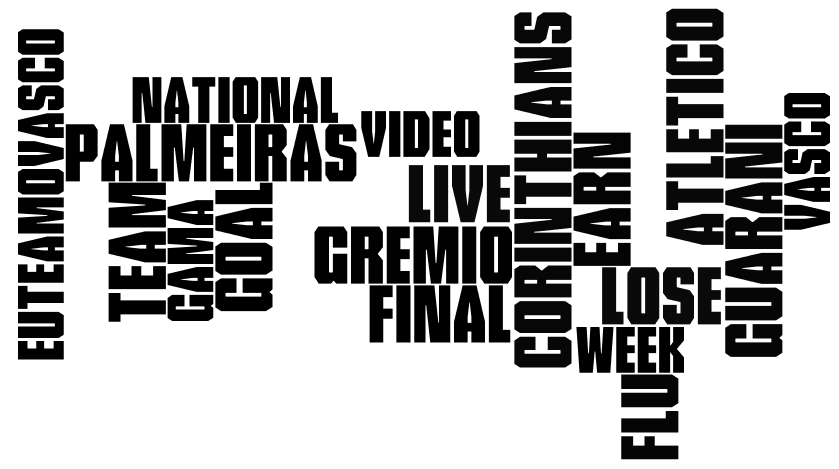
\includegraphics[width=1.5in,height=1.45in]{figures/cloudtags/football.png}}
% \subfigure[Cars]{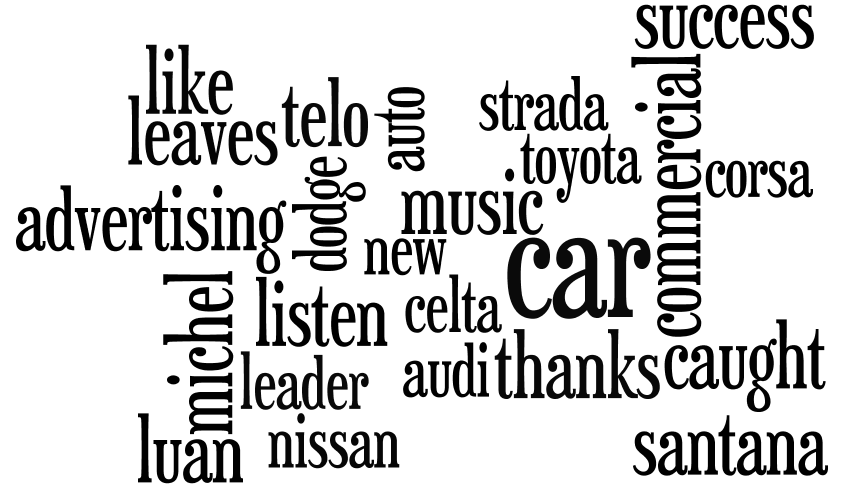
\includegraphics[width=1.5in,height=1.45in]{figures/cloudtags/car.png}}
% \subfigure[Dengue Fever]{
\includegraphics[width=1.5in,height=1.45in]{figures/cloudtags/dengue.png}}
% \subfigure[Politics]{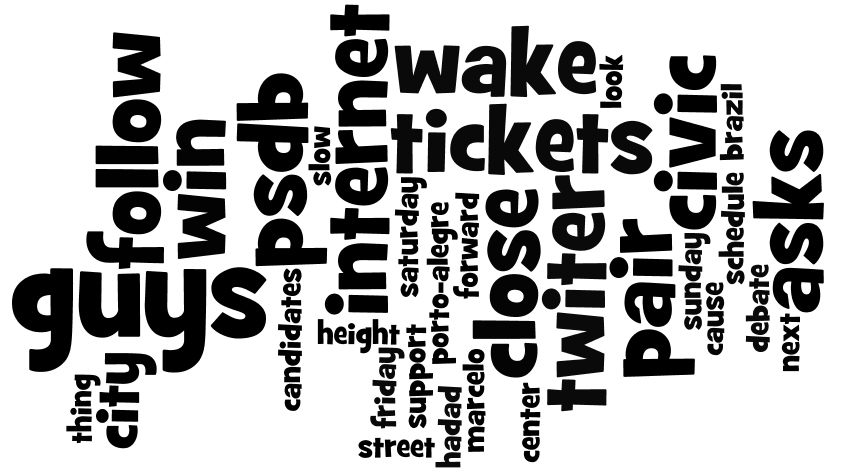
\includegraphics[width=1.5in,height=1.45in]{figures/cloudtags/politics.png}} 
% \caption{Main terms found in the top-4 topics in the Observatory dataset}
% \label{fig:topics}
% \end{figure*}


%However, the best way to evaluate the job being done by the method is to look at the topics generated. Table~\ref{tbl:topicDescriptions} shows the top-15 topics for Observatory and agNews. \gi{comparar com as classes do agnews}

From the results previously discussed, we can conclude that \method presents solutions statistically better than those obtained by the baselines when the value of $\alpha$ is tuned accordingly. The semantics of the topics is also good, but results are omitted here due to space restrictions, and presented in the case study in the next section. More importantly, the proposed framework was conceived to scale to bigger datasets. This is its main advantage over the baselines that aim to reduce the number of topics. While EM is linear in the number of documents $N$, the proposed algorithm depends on the number of latent factors $k$ used to describe $N$ and in the diameter $d$ of the graph. Algorithm 1 has time complexity O($(k-1) \times d \times k^3$), where k-1 is the maximum number of 
iterations.

%\begin{figure}[!th]
%\center
%{file=figures/postFrequencyElection.eps,width=2in,height=1.5in}
%\caption{Post frequency per user for Election}
%\label{fig:election}
%\end{figure}

\subsection{Obama's Followers: A Case Study}

This section presents a case study for characterizing a specific group of Twitter users: Obama's followers. The dataset was collected from July to September 2012. %Figure~\ref{fig:election} shows the post frequency per user in the period. 

Recall that, for this dataset, we do not know the discussed topics. Hence, we evaluated the quality of the generated clusters by using an adaptation of the purity metric defined in Eq. 5. Instead of considering the purity of the clusters with respect to the real class, we evaluate the purity of the terms across different groups, as done in \cite{kao2004mining} with entropy.
The results are shown in Table~\ref{tbl:unlabeled}, and for all three data representativeness used, the results of purity are very similar.

Here we perform a more detailed analysis of how topics are merged and how these merges improve user characterization with semantic topics. For this dataset, 33 iterations of the method were performed. Figure~\ref{fig:election} shows four of the top-ten topics most that characterize 80\% of the users.
The first topics, showed in Figure~\ref{fig:election} (a), characterizes 70.5\% of the users. The topic related to the selection criteria of the users, which was indirectly politics. Its main subject is the Democrats convention in September 2012, which decided to support gay marriage. Note the terms \textit{son} and \textit{dog} are not directly related to the topic, and were added during the merge of almost half of NMF output files. 
Analysing the topics in the earlier levels of the merge, we observe that all merges relate to politics. However, it is interesting to notice that the method actually produces a hierarchy of topics, which will generate single topics if the maximum number of iterations is performed. Correctly choosing where to stop in the hierarchy can give the user the topics at the semantic level he wants. Fine-tuning the stopping criteria is the next step.

The second topic which characterizes users (Figure~\ref{fig:election} (b)) is related to the $4^{th}$ of July. It actually shows terms referring to the independence and others referring to wishes of happy birthday or references to a happy and enjoyable weekend. Here \method merged 9 different topics related to best wishes in various events. The third topic is a merge of two topics referring to the congress and its bills. The fourth topic relates to calls for an anti-racist act. Note that the term \textit{phone}, related to call, was associated to this topic in the NMF output.


%\begin{table}
\caption{Textual Description for the top-10 semantic topics identified for Obama's followers.}\label{tbl:topicDescriptionsObama}
\centering
	\begin{tiny}
	\begin{tabular}{|p{7.8cm}|}\hline
		Top-10 NNMF Semantic Topics \\ \hline \hline
wek,shark,friday,past,fashion,tampa,times,monday,sunday,sumer,starts,busy,wekend,fotbal,ready\\
top,stories,daily,times,ten,\#lastfm,artists,tweted,york,botom,bcvisionweb,gun\\
political,power,ads,politics,history,parties,system\\
akin,tod,race,rep,senate,coments,\#mosen\\
party,tea,democratic,platform\\
election,voter,law,voting,fraud,recal,presidential,voters,wisconsin,early,betwen,important,court,ohio,choice\\
america,bank,comunist,muslim,awake,united,states,anti,bless,destroy,fredom,garbage,founders,stand,nation\\
wrong,place,side,agre,word,sems,fuck,prove,person,law,totaly,speled,policy,question,facts\\
suport,marriage,\#txsen,child,equality,public,conservative,apreciate,congress,proud,govt,act,platform,retwet,sign\\
guy,told,kind,girl,car,runing,funy,heard,pick,rich,hel,asked,smart,face,wanted\\\hline\hline

Top-10 Semantic Topics after 5 iterations of the merging algorithm \\ \hline \hline

put,place,biden,gona,face,chains,line,hands,joe,mouth,word,car,front,charge,pants\\
awesome,sounds,totaly,dude,congrats,gona,wekend,fucking,place,super,amazing,kind,met,movie,glad\\
wrong,place,side,agre,word,sems,fuck,prove,person,law,totaly,speled,policy,question,facts\\
hard,working,hit,worked,die,drive,understand,easy,play,hiting,times\\
political,power,ads,politics,history,parties,system\\
world,life,real,change,climate,pro,shit,estate,rest,center,mind,trade,place,living,record\\
guy,told,kind,girl,car,runing,funy,heard,pick,rich,hel,asked,smart,face,wanted\\
los,times,fun,coming,por,son,idea,del,para,con,las,una,mas,pero,como\\
twiter,stuf,read,post,twet,check,folow,blog,twets,funy,folowers,reading,acount,interesting,found\\
police,dead,facebok,updates,woman,city,election,neds,game,convention,ago,americans,gay,rape,spech\\\hline\hline

Top-10 Semantic Topics after 9 iterations of the merging algorithm \\ \hline \hline

wow,amazing,crazy,shit,beautiful,fox,guess,words\\
put,place,biden,gona,face,chains,line,hands,joe,mouth,word,car,front,charge,pants\\
awesome,sounds,totaly,dude,congrats,gona,wekend,fucking,place,super,amazing,kind,met,movie,glad\\
wrong,place,side,agre,word,sems,fuck,prove,person,law,totaly,speled,policy,question,facts\\
hard,class,midle,working,taxes,rich,hit,worked,die,drive,understand,easy,play,hiting,times\\
caled,place,heard,biden,joe,word,song,reason,told,racist,movie,chris,john,stupid,mom\\
guy,told,kind,girl,car,runing,funy,heard,pick,rich,hel,asked,smart,face,wanted\\
los,times,fun,coming,por,son,idea,del,para,con,las,una,mas,pero,como\\
twiter,stuf,read,post,twet,check,folow,blog,twets,funy,folowers,reading,acount,interesting,found\\
police,dead,facebok,updates,truth,woman,city,election,neds,political,game,convention,ago,americans,gay\\\hline\hline

Top-10 Semantic Topics after 12 iterations of the merging algorithm \\ \hline \hline

col,hot,stay,super,totaly,sumer,air,music,sounds,place,dude,dad,pic,kinda,west\\
story,raw,cover,amazing,ful,told,sad,short,tels,link,interesting,bain,write,breaking,teling\\
wow,amazing,crazy,shit,beautiful,fox,guess,words\\
put,place,biden,gona,face,chains,line,hands,joe,mouth,word,car,front,charge,pants\\
awesome,sounds,totaly,dude,congrats,gona,wekend,fucking,place,super,amazing,kind,met,movie,glad\\
wrong,place,side,agre,word,sems,fuck,prove,person,law,totaly,speled,policy,question,facts\\
friends,wekend,fox,share,met,word,words,close,dear,liberal,enemies,open,conservative,colege,stay\\
talking,points,politics,clint,eastwod,chair,shit,abt,empty,economy,biden,heads,issues,fuck,joe\\
los,times,fun,coming,por,son,idea,del,para,con,las,una,mas,pero,como\\
police,dead,facebok,updates,truth,woman,city,election,neds,political,game,convention,ago,americans,gay\\\hline
\end{tabular}
\end{tiny}
\end{table}







